\documentclass{ltxdoc}

\usepackage{forloop}
\usepackage{pgf}
\usepackage{framed}
\usepackage{holtxdoc}
\usepackage{url}
\usepackage{addlines}
\usepackage[trans={lt, de, en, fa}]{quran}
\usepackage{listings}
\usepackage{tikz}
\usetikzlibrary{calc}
\usepackage{fontspec}
\newfontfamily\quran[Script=Arabic]{Scheherazade}
\hypersetup{%
  plainpages=false,%
  bookmarksnumbered,%
  pdftitle={The quran Package},%
  pdfkeywords={quran, surah, ayah, juz, hizb, ruku, manzil},%
  pdfauthor={Seiied-Mohammad-Javad Razavian},%
  baseurl={http://mirrors.ctan.org/macros/xetex/latex/quran/doc/quran-doc.pdf},%
}
% because of definition of \XeTeX and \XeLaTeX symbols in bidi, I should undef these macro that are also defined in holtxdoc package. 
\makeatletter
\bidi@undef\XeTeX
\bidi@undef\XeLaTeX
\makeatother
\usepackage{bidi}
\makeatletter
\bidi@preto\qurantext{\quran}
\bidi@BeforeBeginEnvironment{declcs}{\vspace*{-4mm}}
%\bidi@AfterEndEnvironment{declcs}{\vspace{-2mm}}
\makeatother

%%%%%%%%%%%%%%%%%%%%%%%%%%%%%%%%%%%%%%%%%%%%%

\def\boxcs#1{\leftline{\fbox{\mcs{#1}}}}
\def\mcs#1{\lr{\texttt{\textbackslash{}#1}}}
\def\tt#1{\lr{\texttt{#1}}}
\lstdefinestyle{BashInputStyle}{
  language=bash,
  basicstyle=\footnotesize\sffamily,
%  numbers=left,
%  numberstyle=\tiny,
%  numbersep=3pt,
  frame=tb,
  columns=fullflexible,
  backgroundcolor=\color{gray!10},
%  linewidth=0.9\linewidth,
%  xleftmargin=0.1\linewidth
}
\def\qp#1{
\begin{minipage}{.6\textwidth}
    #1
\end{minipage}
}

% Define box and box title style
\tikzstyle{mybox} = [draw=black, fill=gray!20, very thick,
    rectangle, rounded corners, inner sep=10pt, inner ysep=20pt]
\tikzstyle{fancytitle} =[fill=gray, text=white]

\def\mx#1#2{\mybox{#1}{#2}{.45\textwidth}}
\def\mxf#1#2{\mybox{#1}{#2}{\textwidth}}

\def\mybox#1#2#3{
\begin{tikzpicture}
\setRTL
\node [mybox] (box){%
    \begin{minipage}[t]{#3}
        #2
    \end{minipage}
};
\node[fancytitle, anchor=west, right=10pt] at (box.north west) {\small \cs{#1}};
\node (hole) [anchor=north east, left=5pt ] at (box.north east) { \tikz\fill[very thick,white] (0,0) circle (12pt); };
\node[ ] at (hole.center) {
\includegraphics[width=.05\textwidth]{quran.png}};
\end{tikzpicture}%
}

%%%%%%%%%%%%%%%%%%%%%%%%%%%%%%%%%%%%%%%%%%%%%

\title{
\includegraphics[scale=.3]{quran.png}\\
The \xpackage{quran} Package\footnote{to one who has devoted his life to Quran}}
\author{Seiied Mohammad Javad Razavian\\\xemail{javadr@gmail.com}}

\date{\qurandate}

\begin{document}
\maketitle

\begin{framed}
This manual is incomplete and the package is under development. \par 
\centerline{\quranversion}
\end{framed}

\tableofcontents
\newpage

\section{Introduction}
This package is prepared for typesetting The Holy Quran%. 
, provides several macros for
typesetting the whole or any parts of The Holy Quran based on its popular division.\footnote{This work is inspired by \xpackage{lipsum} and 
\xpackage{ptext} packages.}
%\footnote{
By recent versions, the package can typeset the translation of The Holy Quran in 
german, english, and persian. It also can typeset quarn transliteration. 
%}\addlines[1]

\section{Loading Package}
You can load the package in the ordinary way
\cs{usepackage[option]\{quran\}}.
After loading the package, it writes some information about itself to the
terminal and to the log file, too. The information is something like:

\begin{lstlisting}[style=BashInputStyle, language=tex, escapechar={|}]
Package: quran |\qurandate| |\quranversion| An easy way to typeset the whole or any part of The Holy Quran
\end{lstlisting}

\section{Typesetting The Holy Quran}\label{sec:qurantypesetting}
For typesetting any parts or whole of The Holy Quran there are several macros in the package.

\subsection{Surah/Sovar}
\begin{declcs}{quransurah}\oarg{m}
\end{declcs}
This macro can typeset any Surah of Quran. As you know there are 114 Sovar, so \textit{m} could 
be an integer between 1 to 114. The macro also could accept the transliteration of surah's name, 
e.g. both of \cs{quransurah[1]} and \cs{quransurah[Al-Fatiha]} have the same effect. For using 
surah's name instead of their order see table~\ref{tab1}.
\marginpar{\cs{quransurah[1]}}\marginpar{\cs{quransurah[Al-Fatiha]}}
    \centerline{\hbox{\mx{quransurah[94]}{\quransurah[94]}\hfill
    \mx{quransurah[At-Tin]}{\quransurah[At-Tin]}}}
    
\begin{declcs}{quransurah}\oarg{m-n}
\end{declcs}
This acts like above but can typeset \textit{m}$^{th}$ Surah to \textit{n}$^{th}$  one. 

\begin{declcs}{quransurah}\oarg{m{-}{-}n}
\end{declcs}
In this case m and n are tranliterations of surah's names, e.g. \cs{quransurah[An-Nasr--An-Nas]}.
\marginpar{\cs{quransurah[An-Nasr--An-Nas]}}

    \centerline{\hbox{\mx{quransurah[109-110]}{\quransurah[109-110]}\hfill
    \mx{quransurah[Al-Masadd--Al-Ikhlas]}{\quransurah[Al-Masadd--Al-Ikhlas]}}}
    
\newcounter{ct}
\def\mycell#1{
    \surahname[\value{#1}]
    \addtocounter{#1}{38}
}
\begin{table}[tbhp]
    \centering
    \fontsize{8}{10}\selectfont
    \begin{tabular}{|*{3}{c|l|}}
    \hline
     order & surahname & order  & surahname  & order  & surahname  \\
    \hline\hline%
    \forloop{ct}{1}{\value{ct} < 38}{%
        \thect & \mycell{ct} & \thect & \mycell{ct} & \thect & \mycell{ct}  \\
        \addtocounter{ct}{-114}
    }%
    \thect & \mycell{ct} & \thect & \mycell{ct} & \thect & \mycell{ct}\\%
    \hline
    \end{tabular}
    \protect\caption{Surah's name trasliteration.}\label{tab1}
\end{table}
    

\begin{declcs}{quransurah}
\end{declcs}
Using \cs{quransurah} without its optional argument typeset the default Surah--Al-Ikhlas.

\centerline{\mx{quransurah}{\quransurah}}

To change the default Surah use \cs{setsurahdefault\{m\}}, again m must be between 1 and 114; 
as know noticed package's default is 112.
\marginpar{\cs{setsurahdefault}}

After changing package's default surah to 107 by \cs{setsurahdefault\{107\}}, the output would be like below:

    \setsurahdefault{107}
    \centerline{\mx{quransurah}{\quransurah}}



\subsection{Ayah/Ayat}
\begin{declcs}{quranayah}\oarg{l}\oarg{n}
\end{declcs}
The above macro typeset the \textit{n}$^{th}$ Ayah of \textit{l}$^{th}$ Surah. 

    \centerline{\hbox{\mx{quranayah[33][33]}{\quranayah[33][33]}\hfill
    \mx{quranayah[Al-Ahzab][33]}{\quranayah[Al-Ahzab][33]}}}
    
If you just typeset the first Ayah of any Surah, then the Basmalah will not be printed.
In this case if you need Basmalah, then you can use the \cs{basmalah} macro before.
\marginpar{\cs{basmalah}}

    \centerline{\hbox{\mx{quranayah[Ibrahim][1]}{\quranayah[Ibrahim][1]}\hfill
    \mx{basmalah\textbackslash{}quranayah[14][1]}{\quran\basmalah\quranayah[14][1]}}}

\begin{declcs}{quranayah}\oarg{l}\oarg{m-n}
\end{declcs}
This macro typeset the \textit{m}$^{th}$ to \textit{n}$^{th}$ Ayat of l$^{th}$ Surah. 

\par
\addvspace{4.5ex plus 1ex}%
\vskip -\parskip
\noindent\textit{l} could be an integer less than or equal to 114. It also could be 
the transliteration of  l$^{th}$ Surah's name, see table~\ref{tab1}. 
\textit{n} is diffirent by every Surah and it relies on the number of the Surah's verses. 
\textit{m} should be between 1 and a number less than \textit{n}. 

In case of using tranliteration of surah's name, both \cs{quransurah} and \cs{quranayah} are \emph{case-insensitive}, i.e. 
for example there is no differences between Al-Fatihda, al-fatiha, al-Fatiha, 
 and any other possible combinations of lowercase and uppercase letters.

    \centerline{\hbox{\mx{quranayah[Ash-Shura][22-26]}{\quranayah[Ash-Shura][22-26]}\hfill
    \mx{quranayah[42][22-26]}{\quranayah[42][22-26]}}}

\subsection{Page/Pages}
\begin{declcs}{quranpage}\oarg{n}
\end{declcs}
Typeset the \textit{n}$^{th}$ page of Quran and the macro below typeset \textit{m}$^{th}$ to 
\textit{n}$^{th}$ pages of Quran. 

\begin{declcs}{quranpage}\oarg{m-n}
\end{declcs}
The numbers should be between $1$ to $604$, based on Uthmani text. 

    \centerline{\hboxR{\mx{quranpage*[249]}{\quranpage*[249]}
    \hfill
    \mx{quranpage*[250]}{\quranpage*[250]}}}
    
    * starred version of macros are explained in page~\pageref{starred}; concisely it means
    typesetting that part of the Holy Quran in one paragraph. 
    
    \centerline{\mxf{quranpage*[1-3]}{\quranpage*[1-3]}}
    
\subsection{Juz/Ajza}
%\vspace{-6mm}
\begin{declcs}{quranjuz}\oarg{n}
\end{declcs}
Above macro typesets the \textit{n}$^{th}$ juz of Quran and below macro typesets m$^{th}$ to n$^{th}$ juzzes of Quran. 

\begin{declcs}{quranjuz}\oarg{m-n}
\end{declcs}
%\vspace{-6mm}
The numbers should be between $1$ to $30$.

\subsection{Hizb/Ahzab}
Each juz of Quran is devided into two ahzab (group),  so there are 60 ahzab.
Following macros typeset hizb/ahzab of Quran. 

%\vspace{-6mm}
\begin{declcs}{quranhizb}\oarg{n}
\end{declcs}
%\vspace{-14mm}
\begin{declcs}{quranhizb}\oarg{m-n}
\end{declcs}


\subsection{Quarter/Quarters}
Eash hizb of Quran is devided into four quarters, making eight quarters per juz, called maqra. 
There are 240 of these quarters (of hizb) in the Quran. These maqra are often used as sections for revision when memorizing the Quran.\footnote{\url{https://en.wikipedia.org/wiki/Juz'}}

%\vspace{-6mm}
\begin{declcs}{quranquarter}\oarg{n}
\end{declcs}
%\vspace{-14mm}
\begin{declcs}{quranquarter}\oarg{m-n}
\end{declcs}

Above macros typeset the \textit{n}$^{th}$ or m$^{th}$ to n$^{th}$ quarter(s) of Quran.   

    \centerline{\mxf{quranquarter*[110]}{\quranquarter*[110]}}
    
\subsection{Ruku/Rukus}
``The term ruk\= uʿ --- roughly translated to ``passage", ``pericope" or ``stanza" --- is also used to denote a group of thematically related verses in the Qur'an. Longer suras (chapters) in the Qur'an are usually divided into several ruk\= us, so that the reciters could identify when to make ruk\= u in Salat without breaking an ongoing topic in the Quranic text."\footnote{\url{https://en.wikipedia.org/wiki/Ruku}}

The following macros can typeset rukus of The Holy Quran the way the above macros act. 

\begin{declcs}{quranruku}\oarg{n}
\end{declcs}

    \centerline{\mxf{quranruku*[363]}{\quranruku*[363]}}
    
\begin{declcs}{quranruku}\oarg{m-n}
\end{declcs}
The numbers should be between $1$ to $556$.

    \centerline{\mxf{quranruku*[58-59]}{\quranruku*[58-59]}} 

    
\subsection{Manzil/Manazil}
``For the convenience of people who wish to read the Qur'an in a week the text may be divided into 7 portions, each portion is known as Manzil.

The following division to 7 equal portions is by Hamza Al-Zayyat (d.156/772):
\begin{enumerate}
    \item Al-Fatihah (chapter 1) through An-Nisa' (chapter 4) consisting of 4 surahs.
    \item Al-Ma'ida (chapter 5) through At-Tawba (chapter 9) consisting of 5 surahs.
    \item Yunus (chapter 10) through An-Nahl (chapter 16) consisting of 7 surahs.
    \item Al Isra' (chapter 17) through Al-Furqan (chapter 25) consisting of 9 surahs.
    \item Ash-Shuara' (chapter 26) through Ya-Seen (chapter 36) consisting of 11 surahs.
    \item As-Saaffat (chapter 37) through Al-Hujarat (chapter 49) consisting of 13 surahs.
    \item Qaf (chapter 50) through An-Nass (chapter 114) consisting of 65 surahs.''\footnote{\url{https://en.wikipedia.org/wiki/Manzil}}
\end{enumerate}

Following macros typeset manzil/manazil of Quran.

\begin{declcs}{quranmanzil}\oarg{n}
\end{declcs}
%\vspace{-12mm}
\begin{declcs}{quranmanzil}\oarg{m-n}
\end{declcs}

\subsection{Text of Quran}
The following macro is the heart of all macros that can typeset any range of Quran. As you know there 
are $6236$ Ayat in Quran. This macro can typeset a specific Ayah or any range of Ayat. 

\begin{declcs}{qurantext}\oarg{n}
\end{declcs}
Typesets the \textit{n}$^{th}$ Ayah of Quran. 

\centerline{\mxf{qurantext[1023]}{\begingroup\qurantext[1023]\endgroup}}

\begin{declcs}{qurantext}\oarg{m-n}
\end{declcs}
Typesets any range of Ayat from the \textit{m}$^{th}$ to \textit{n}$^{th}$ Ayah. 

    \centerline{\mxf{qurantext*[4111-4117]}{\begingroup\qurantext*[4111-4117]\endgroup}}
 
Using \cs{qurantext} without its optional argument typeset [1-7] --Al-Hamd. To
change the default text use \cs{setqurantextdefault\{m-n\}}
\marginpar{\cs{qurantext}}


    \centerline{\mx{qurantext}{\qurantext}}
    
    \noindent below, the default is changed to \cs{setqurantextdefault\{4128-4147\}}:
    \marginpar{\cs{setqurantextdefault\{m-n\}}}
    
    \setqurantextdefault{4128-4147}
    \centerline{\mxf{qurantext*}{\qurantext*}}

\subsection{Whole of The Holy Quran}
The following macros can typeset whole of The Holy Quran:

\begin{itemize}
    \item \cs{quransurah[1-114]}
    \item \cs{quranjuz[1-30]}
    \item \cs{quranpage[1-604]}
    \item \cs{qurantext[1-6236]}
    \item \cs{quranhizb[1-60]}
    \item \cs{quranquarter[1-240]}
    \item \cs{quranruku[1-556]}
    \item \cs{quranmanzil[1-7]}
\end{itemize}

\section{Miscellaneous}

\subsection{Name of Surah}
\begin{declcs}{surahname}\oarg{m}
\end{declcs}
This macro returns the tranliteration of \textit{m}$^{th}$ Surah.

\begin{declcs}{surahname*}\oarg{m}
\end{declcs}
This macro returns the arabic name of \textit{m}$^{th}$ Surah.

    \centerline{\hbox{\mx{surahname[19]}{\surahname[19]}
    \hfill
    \mx{surahname*[19]}{\quran\surahname*[19]}}}
    
\subsection{Basmalah}
\begin{declcs}{basmalah}
\end{declcs}
It provides the basmalah in arabic text which every Surah is started by that.

    \centerline{\mx{basmalah}{\quran\basmalah}}
    
\subsection{Index Converting}
\begin{declcs}{indexconvert}\marg{index}\marg{surah macro}\marg{ayah macro}
\end{declcs}
This command converts an index number between 1 to 6236 
to its exact surah's index and ayah's index. The index must be a number or
\TeX{} counter, the surah macro and ayah macro must be \TeX{} macro names. They
will be set to numbers representing the surah and ayah of the given index in whole of Quran.

\section{Options to The Package}
All text generated by macros of this package will be separated by the macro \cs{par}. Sometimes, 
a version of text without \cs{par} is desired. Therefore the package provides the option 
\texttt{nopar}\marginpar{\texttt{nopar}}
that causes no macros of the package terminated by \cs{par}.
Another way for achieving this, is using the starred version of macros. All macros of the package
has a starred version that omit the \cs{par} macro in typesetting the text of Quran. 

\label{starred}
In some cases maybe user wants to typeset the Ayat without their following numbers that can be seen in printed version of The Holy Quran. The \texttt{nonumber}\marginpar{nonumber} 
option tells the package that print no number after ayah.
But sometimes we want to typeset just some Ayat without theirs, so there is a \cs{ToggleAyahNumber} macro
that can cause numbers will be omitted. With \texttt{nonumber} option this macro acts vice versa, it mean it 
causes that Ayat number will be printed.

    \centerline{\mxf{ToggleAyahNumber\textbackslash{}quransurah*[89]}
    {\ToggleAyahNumber\quransurah*[89]}}  
    
By default, the package typesets the text of The Holy Quran in simple script, but if you prefer the Uthmani script you can use \texttt{uthmani} \marginpar{uthmani} 
option. Compare the following text to figure out the differences between default and uthmani script.
    \centerline{\hbox{
    \mx{quransurah*[1] (default)}{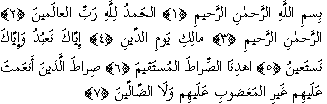
\includegraphics{defaulttext.pdf}}
    \hfill
    \mx{quransurah*[1] (uthmani)}{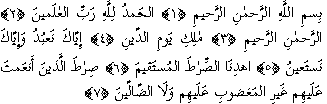
\includegraphics{uthmanitext.pdf}}
    }}
    
By version 1.3, the package can typeset the transliteration of The Holy Quran. 
This option will be useful for whom doesn't really know how to read the arabic text. By loading \texttt{translt}
option all macros that defined in section~\ref{sec:qurantypesetting} will have an ``\texttt{lt}" version. In other words, 
this will add the following macros:
\marginpar{translt} 

\begin{itemize}

    \item \cs{quransurahlt}
    \item \cs{quranayahlt}
    \item \cs{quranpagelt}
    \item \cs{quranjuzlt}
    \item \cs{quranhizblt}
    \item \cs{quranquarterlt}
    \item \cs{quranrukult}
    \item \cs{quranmanzillt}
    \item \cs{qurantextlt}
\end{itemize}

    \centerline{\mx{quransurahlt[108]}{\setLTR\quransurahlt[108]}
    \hfill
    \mx{quransurah[108]}{\quransurah[108]}}
    


By version 1.4, the package can typeset the translation of The Holy Quran in germany, english, and persian. 
\marginpar{transde}\marginpar{transen}\marginpar{transfa}%
These options added because of some requests from users who need the translation of The Holy Quran in their languages. 
By loading \texttt{transde}, \texttt{transen}, and \texttt{transfa} the package can typeset the translation in 
 germany, english, and persian, respectively.

By loading echo of these options, all macros that defined in section~\ref{sec:qurantypesetting} will have 
a ``\texttt{de}"/``\texttt{en}"/``\texttt{fa}"  version. In other words, 
thsee will add the following macros:


\begin{multicols}{3}
\texttt{transde} option:
\begin{itemize}
    \item \cs{quransurahde}
    \item \cs{quranayahde}
    \item \cs{quranpagede}
    \item \cs{quranjuzde}
    \item \cs{quranhizbde}
    \item \cs{quranquarterde}
    \item \cs{quranrukude}
    \item \cs{quranmanzilde}
    \item \cs{qurantextde}
\end{itemize}

\texttt{transen} option:
\begin{itemize}
    \item \cs{quransurahen}
    \item \cs{quranayahen}
    \item \cs{quranpageen}
    \item \cs{quranjuzen}
    \item \cs{quranhizben}
    \item \cs{quranquarteren}
    \item \cs{quranrukuen}
    \item \cs{quranmanzilen}
    \item \cs{qurantexten}
\end{itemize}

\texttt{transfa} option:
\begin{itemize}
    \item \cs{quransurahfa}
    \item \cs{quranayahfa}
    \item \cs{quranpagefa}
    \item \cs{quranjuzfa}
    \item \cs{quranhizbfa}
    \item \cs{quranquarterfa}
    \item \cs{quranrukufa}
    \item \cs{quranmanzilfa}
    \item \cs{qurantextfa}
\end{itemize}
\end{multicols}
    
    All translations are from \url{tanzil.net}. For germen, english, and persian languages the ``Abu Rida Muhammad ibn Ahmad ibn Rassoul", ``Ahmed Ali", ``Mohammad Mahdi Fooladvand" is choosen respectively, by suggestion of the package's users.
    
    Another option is defined that simplifies the usage of mutiple translations simultaneously. The \texttt{trans} option can get 
    any permutation of  ``\texttt{lt}", ``\texttt{de}", ``\texttt{en}", and ``\texttt{fa}". e.g. this document loads the \texttt{quran} 
    package with ``\texttt{trans=\{lt, de, en, fa\}}" option. 
    \marginpar{trans}  
        
    \centerline{\mx{quransurahfa[108]}{\quransurahfa[108]}
    \hfill
    \mx{quransurah[108]}{\quransurah[108]}} 
    \centerline{\mx{quransurahen[108]}{\setLTR\small\quransurahen[108]}
    \hfill
    \mx{quransurahde[108]}{\setLTR\small\quransurahde[108]}}
    

\section{Acknowledgment}
At first, I should appreciate Vafa Khaligi by preparing such adorable packages --\xpackage{bidi} and 
\xpackage{xepersian}. Secondly, the costly \url{http://tanzil.net/} for providing the text of The Holy Quran that 
is developed by Hamid Zarrabi-Zadeh. And finally, people in Parsi\LaTeX\footnote{\url{http://parsilatex.com/}}
group who tested and commented this work in advance. 

\section{Frequently Asked Questions}
    \subsection{What is the best font for typesetting quran text?}
    We strongly recommend you to use "Scheherazade"%
    \footnote{\url{http://software.sil.org/scheherazade/}} 
    and "Amiri"% 
    \footnote{\url{http://www.amirifont.org/}} fonts.

    Scheherazade is released under the SIL Open Font License (OFL), version 1.1. Copyright (c) 2004-2015,
    SIL International (http://scripts.sil.org/) with Reserved Font Names "Scheherazade" and "SIL". Therefore
    you can freely download it. 
    All examples in this document use this font.  
    
    Amiri is a classical Arabic typeface in Naskh style for typesetting books and other running text.
    Amiri is a revival of the beautiful typeface pioneered in early 20th century by Bulaq Press in Cairo, 
    also known as Amiria Press, after which the font is named.
    Amiri is a free, open source project that everyone is encouraged to use and modify.
    
    \subsection{How to use \xpackage{quran} package?}
    As you've noticed, for typesetting quran text you need a package that can typeset text
    in RTL mode in additon to using UTF8 fonts, because \xpackage{quran} draws its text from a 
    unicoded databases. The \xpackage{polyglossia}, 
    \xpackage{fontspec}, and \xpackage{bidi} will do that for you. 
    You can also use \xpackage{xepersian} that relies on \xpackage{fontspec}, too. 
    Another choices are \xpackage{arabxetex} and \xpackage{arabluatex} that the latter just 
    works with  \LuaLaTeX{} while former 
    ways work with \XeLaTeX. \xpackage{arabxetex} and \xpackage{arabluatex}  use Amiri font by default. 
    The following demonstrates  examples for all four approaches:

\begin{lstlisting}[style=BashInputStyle, language=tex, title=``example: with polyglossia{,} 
fontspec{,} and bidi"]
\documentclass{article}

\usepackage{quran}

%%% for typesetting arabic text
\usepackage{polyglossia}
\setotherlanguage{arabic}

\usepackage{fontspec}
\setmainfont{Scheherazade}

%%% for typesetting in Rigth-To-Left direction
\usepackage{bidi}

\begin{document}

\setRTL % tell bidi to typeset the text in Rigth-To-Left direction
\textarabic{\quransurah}

\end{document}
\end{lstlisting}    
    

\begin{lstlisting}[style=BashInputStyle, language=tex, title=``example: with xepersian"]
\documentclass{article}

\usepackage{quran}

%%% for typesetting Persian/Arabic text in Rigth-To-Left direction
\usepackage{xepersian}
\settextfont{Scheherazade}

\begin{document}

\quransurah

\end{document}
\end{lstlisting}  

\begin{lstlisting}[style=BashInputStyle, language=tex, title=``example: with arabxetex"]
\documentclass{article}

\usepackage{arabxetex} % for typesetting Arabic text in Rigth-To-Left direction
\usepackage{quran}

\begin{document}

\begin{arab}[utf]
    \quransurah
\end{arab}

\end{document}
\end{lstlisting} 

\begin{lstlisting}[style=BashInputStyle, language=tex, title=``example: with arabluatex"]
\documentclass{article}

\usepackage{arabluatex} % for typesetting Arabic text in Rigth-To-Left direction
\usepackage{quran}

\begin{document}

\begin{txarab}
    \quransurah
\end{txarab}

\end{document}
\end{lstlisting} 
    
    \subsection{How to set quran default font?}
        If you want to automatically change the font of quran text in your document, you 
        can put your willing font in precede of \cs{qurantext} like below:
        
        In case you are using \xpackage{xepersian}, put below commands in preamble:
        
\begin{lstlisting}[style=BashInputStyle]
\defpersianfont\quran{Scheherazade}
\makeatletter
\bidi@preto\qurantext{\quran}
\makeatother
\end{lstlisting}

    In case you are using \xpackage{fontspec}, put below commands in preamble:
\begin{lstlisting}[style=BashInputStyle]
\usepackage{etoolbox}
\newfontfamily\quran{Scheherazade}
\preto\qurantext{\quran}
\end{lstlisting}

    By setting default font as above, if you want to use \cs{quratext}, you have to enclose it in curly braces. If you don't, 
    it will affect the following text font. 
\begin{lstlisting}[style=BashInputStyle]
{\qurantext[x-y]}
\end{lstlisting}    
    \subsection{How to typeset a portion of the Holy Quran in one paragraph
    with no ayah number without affecting the behaviour of \xpackage{quran} package 
    in other cases?}
    
    Just put the code that was describled on page~\pageref{starred} in a group like:
\begin{lstlisting}[style=BashInputStyle]
{\ToggleAyahNumber\quransurah*}
\end{lstlisting}    

\end{document}
